\documentclass[preprint]{sigplanconf}


\usepackage{amsmath}
\usepackage{amsthm}
\usepackage{amssymb}
\usepackage{stmaryrd}
\usepackage[pdftex]{graphicx}

% Margin notes (ugly and complicated)
%% \usepackage[draft]{fixme}
%% \fxusetheme{color}
%% %\fxusetheme{signature}
%% %\fxuselayouts{pdfmargin}
%% %\fxusetargetlayout{color}
%% \FXRegisterAuthor{nc}{anc}{NC}

% Margin notes round two (easier and better looking)
%
% http://trackchanges.sourceforge.net/help_stylefile.html
%
% NB: if you want to add a note in math mode, you need a trick:
%
% $ ... \text{\note{$<math note>$}} ... $
\usepackage[inline]{trackchanges} % [margins] is also good
\addeditor{nc}

\begin{document}

\def\ruleform#1{{\setlength{\fboxrule}{1.2pt}\fbox{\normalsize $#1$}}}
\newcommand{\dtrans}[1]{\mathcal{D} \llbracket #1 \rrbracket}
\newcommand{\ktrans}[1]{\mathcal{K} \llbracket #1 \rrbracket}
\newcommand{\ctrans}[1]{\mathcal{C} \llbracket #1 \rrbracket}
\newcommand{\trans}[1]{\llbracket #1 \rrbracket}

\newcommand{\tot}{\leftrightarrow}

\newtheorem{definition}{Definition}

%% We could use \texttt{true} and \texttt{false} here, to be more
%% consistent with \bad and \unr, but then we should also use
%% \texttt{Nil}, \texttt{Cons}, etc.
\newcommand{\true}{True}
\newcommand{\false}{False}
\newcommand{\unr}{\texttt{UNR}}
\newcommand{\bad}{\texttt{BAD}}
\newcommand{\any}{\texttt{Any}}
\newcommand{\ok}{\texttt{Ok}}
\newcommand{\hprime}{\ensuremath{\mathcal{H}'}}
% Full function application, e.g. $\full{f}(x_1,\ldots,x_n)$. Contrast
% with partial application, e.g. $f~x_1 \ldots x_n$
\newcommand{\full}[1]{\hat{#1}}
\newcommand{\cfc}{\texttt{CF}}
\newcommand{\cf}[1]{\texttt{CF}(#1)}
\renewcommand{\min}[1]{\mbox{min}(#1)}

\newcommand{\designChoice}{(DESIGN CHOICE/OPTIONAL)}

\title{Static contract checking for Haskell}
\authorinfo{Simon, Koen, Dimitrios, Charles-Pierre}
\maketitle

\section{Introduction}

Our approach to static contract-checking is to translate source code
to a first-order logic theory and
 then use an automated theorem prover
to check the consistency of the theory.

Consider:\note[nc]{Unlike the POPL '09 paper, $\cf{e}$ is not implied by $e \in \{x|p\}$.}
\begin{verbatim}
data List = Nil 0 | Cons 2

notnull x = case x of
  Nil -> False
  Cons x y -> True

head ::: (CF && {x | notnull x }) -> CF
head xs = case xs of
  Nil -> BAD
  Cons x y -> x
\end{verbatim}

First, we need to encode the List structure. 

We start by stating that $Nil$ and $Cons$ can never be equal:
\begin{equation*}
\forall a,b.~Cons~a~b \neq Nil
\end{equation*}

Then, we state that $Nil$ can cannot cause a crash, and that
$Cons~x~y$ cannot cause a crash iff both its arguments cannot. The
statement ``$x$ cannot cause a crash'' is encoded by the formula
$\cf{x}$.\note[nc]{I just rewrote this, but it still sounds weird: in
  $head~Nil = \bad$, who ``caused'' the crash? The precise definition
  of $\cf$ in Section \ref{sec:cf}, in terms of not leading to crashes
  when inserted into syntactically \bad-free environments,  is good, but
  how to state it informally?}

\begin{equation*}
\cf{Nil}
\end{equation*}
\begin{equation}
  \label{cfcons}
\forall a,b.~\cf{a} \land \cf{b} \iff \cf{Cons~a~b}
\end{equation}

We also say some stuff about \annote[nc]{unreachibility}{??? e.g. \[
  CF(fst~(x,BAD)) \iff CF(x) \] as in section \ref{sec:cf}?} but I
can't think of a good way to explain it right now.
\begin{equation*}
\forall y,ys.~Cons~y~ys \neq \unr
\end{equation*}
\begin{equation*}
Nil \neq \unr 
\end{equation*}\note[nc]{\unr means ``infinite loop'', approximately (it's also the result of pattern matches on non-loop expressions with the wrong constructor head), and so these rules ($\phi_\text{lazy}$) say that constructors are ``lazy'' or ``total''.}

Finally, we define projections for $Cons$. \annote[nc]{It is not
  strictly necessary, but it will be handy:}{??? Why is it handy? It
  doesn't seem to play any role in formal part of this paper (besides
  being specified in axioms $\phi_\text{projection}$). In the current
  implementation it's used to avoid introducing existentially
  quantified variables in the $\bigvee_i$ part of $\dtrans{}$ for
  functions defined by case expressions. Equation \eqref{unrnotnull}
  below uses it that way. ??? Does Equinox care?}
\begin{equation*}
\forall xs,y,ys.~sel_{1,Cons}~Cons~y~ys = xs \implies xs = y 
\end{equation*}
\begin{equation*}
\forall xs,y,ys.~sel_{2,Cons}~Cons~y~ys = xs \implies xs = ys 
\end{equation*}\note[nc]{??? Why not the simpler \[\forall y,ys.~sel_{2,Cons}~Cons~y~ys = ys\]? Same question in Figure \ref{dtrans}.  (Equinox does have a built in notion of equality, e.g. running equinox on
\center{\texttt{fof(\_,theorem,? [X,Y] : (X = Y \& f(X) != f(Y))).}}\\
 results in ``Unsatisfiable'', so support for equality reasoning is not the reason.)}
%% \[
%% \text{\texttt{\$ echo "fof(\_,theorem,? [X,Y] : (X = Y & f(X) != f(Y)))."}} \\
%%                  \text{\texttt{| equinox /dev/stdin}}}}
%% \]

Now we translate the $null$ function.
\begin{equation*}
\forall xs.~ xs=Nil \implies notnull~xs = \false
\end{equation*}\note[nc]{Here we might ask the same question as above: why not use the simpler definition
\[
notnull~Nil = \false
\]? The answer is that this is an expansion of the $e = K_i~\vec{x_i} \to a = e_i$ part of the $\dtrans{}$ rule for functions defined by cases.  I.e., the scrutinee $Nil$ is, in general, an expression involving, but not necessarily equal to, the arguments to the function.  In this special case we could remove the implication, but not in general.  The $a = e_i$ part is missing above, but I guess that's because this text was not updated for the $\min$-translation.}

\begin{equation}
  \label{defnotnull}
\forall xs,y,ys.~ xs=Cons~y~ys \implies notnull~xs = \true
\end{equation}

We also need to specify the translation of calls to $notnull$ with
$\bad$ values, to encode the fact that $notnull~\bad = \bad$.
\begin{equation*}
\forall xs.~xs=\bad \to notnull~xs = \bad
\end{equation*}

Finally, we say that one call $notnull$ with a an argument which is
not $Nil$ or $Cons$ or $\bad$ then the result is $\unr$.
\begin{align}
  \label{unrnotnull}
  \forall xs.~xs \neq \bad \land xs \neq Nil  \notag \\
  \land xs \neq Cons~(sel_{1,Cons}~xs)~(sel_{2,Cons}~xs) \to  \notag \\
  notnull(xs) = \unr 
\end{align}

The translation of $head$ follows the same pattern:
\begin{align}
  \forall xs.~ x=Nil \implies head~xs = \bad \notag\\
  \forall xs,y,ys.~ xs=Cons~y~ys \implies head~xs = y     \label{defhead} \\
    \forall xs.~xs=\bad \to head~xs = \bad \notag
\end{align}\note[nc]{??? Why not use the same project+construct trick from the last equation?  I.e., why not
\[
\forall xs.~ xs=Cons~(sel_{Cons,1}~xs)~(sel_{Cons,2}~xs) \implies head~xs = sel_{Cons,1}~xs
\]?  Because it's ugly?  Would Equinox care?}

\begin{align*}
 \forall xs.~xs \neq \bad \land xs \neq Nil \notag \\
 \land xs \neq Cons~(sel_{1,Cons}~xs)~(sel_{2,Cons}~xs) \to  \notag \\
 head~xs = \unr
\end{align*}

We now have translated the source code. Let us call all those formulae
the theory $T$. We translate separatly the contract:
\begin{equation*}
  \phi := \forall xs.~\cf{xs} \land notnull~xs = \true \to \cf{head~xs} 
\end{equation*}

Now that we translated everything to first-order logic, we can ask the
theorem prover if the theory formed by those formulae \change[nc]{is
consistent}{entails the contract}, ie if $T \vdash \phi$.

Intuitively, $T$ is consistent (ie $T \not \vdash \bot$), because each
formula serves a specific purpose.\note[nc]{

  A more precise consistency argument by exhibiting a model for $T$:
  in the model we define $\min{}$ to be the trivial predicate,
  i.e. $\forall x. \min{x}$.  So, we can drop all the $\min{}$'s.  The
  model for the resulting formulas is a language with the syntax used
  in this paper ($\mathcal{H}'$ below).

  The carrier consists of all closed (i.e. variable free / grounded)
  programs that can be written using the functions and constructors in
  $T$, using the expression syntax of $\mathcal{H}'$ below, and
  evaluated as described in the following paragraphs.  We assume $T$
  comes from a ``well-typed'' source program $P$, i.e. s.t. the
  Haskell program corresponding to $P$ is well-typed.

  The semantics are what you would expect for ``well-typed''
  terminating expressions (again, ``well-typed'' in the sense that the
  corresponding Haskell expression is well-typed in an environment
  including $P$'s decls). For example, \texttt{Cons~Z~Nil} is
  ``well-typed'' but \texttt{Cons~Nil~Z} is ``ill-typed'' in a the
  context of a program declaring List and Nat types.  

  In general, scrutinizing a \unr{} yields \unr, as does scrutinizing
  a terminating expression with the wrong constructor head
  (e.g. \texttt{tail~(S Z) =} \unr{}). Scrutinizing an ill-typed
  expression with a constructor head of the right type evaluates as
  specified by the pattern (e.g. \texttt{tail~(Cons~Nil~Z) = Z}),
  unless there is no corresponding pattern (``non-exhaustive
  pattern''), in which case the result is \bad{}.  NB: wrong-type and
  no-corresponding-pattern are treated very differently.  The
  intuition is that the former never happens in a well-typed program.

  Applying \unr{} or \bad{} as a function results in \unr{} or \bad{},
  respectively.

  Term constructors have disjoint ranges, and are total.

  I think that covers functions and datatypes, but it remains to argue
  that the axioms for contracts are consistent \ldots.  

  \ldots but maybe this is tricky?  Modeling $CF(e)$ seems easy,
  i.e. just ask the oracle used above for evaluation if $e$ is \bad{}
  or not.  But recursion seems problematic, since we get to assume in
  $T$ that the contract holds in the recursive position (Section
  \ref{sec:recursiveContracts}), and so it seems we need to argue that
  \emph{all} expressable contracts are consistent.

  Here's a flawed contradiction ``proof'': consider
  \[
  e = e ::: CF \&\& \lnot CF.
  \]
  Now, $T$ will contain $CF(ep) \land \lnot CF(ep)$, and were hosed.
  This is flawed because there is no $\lnot$ in the annotated
  contracts.

  OK, and actually this might be easy: we simply interpret all
  recursive function symbols (the $fp$'s for recursive $f$'s) as
  \unr{}, and use the fact that forall $x$, $\unr{}~x = \unr$.  Now,
  an easy induction on contract translations (Figure \ref{ctrans})
  gives \[ \emptyset \vdash \ctrans{\unr \in c} \]\note[nc]{

    Actually, this was not true!  We need an axiom saying $\cf{\unr}$.
    There was already such an axiom in the implementation, but it
    wasn't mentioned in this draft.  So, the correct statement is more
    like
    \[ \text{The Prelude} \vdash \ctrans{\unr \in c} \]

  } for all contracts $c$, and we're done!  Well, this is really just
  the base case, where all contracts in $T$ are for otherwise
  undefined recursion symbols ($fp$'s), but the inductive case is just
  as easy: given a consistent $T$, which may include contracts for
  defined symbols, we can always extend it to a consistent $T'$ by
  adjoining constracts for undefined symbols.

}

Now, assume that $xs$ satisfies
$\cf{xs}$ and $notnull~xs = \true$.  We can derive that $xs \neq \bad$
because we have $\cf{xs}$ and \annote[nc]{$\lnot \cf{\bad}$}{

Follows from the definition of $CF$, but it's worth noting that this
plays a key part in the axiomitization of $CF$.

}. The constraint
$notnull~xs = \true$ doesn't directly imply that $xs = Cons~y~ys$ for
some $y$ and $ys$. But $notnull$ is totally defined, because of
\eqref{unrnotnull}. This implies (by \eqref{defnotnull}) that there exist
$y$ and $ys$ such that $xs = Cons~y~ys$. Recalling $\cf{xs}$, we can
now derive $\cf{y}$ and $\cf{ys}$ (by \eqref{cfcons}). But $head~xs =
y$ because of \eqref{defhead}, and $y$ is crash-free, so we can finally
derive $\cf{head~xs}$. QED.


\section{Languages}
\subsection{$\hprime:~\lambda$-calculus variant}

The syntax of $\mathcal{H}'$ is defined in figure~\ref{hprime-stx}. A module
is a list of toplevel definitions, claims that functions statisfy
contracts and data definitions.

\begin{itemize}
\item There's no $\lambda$-abstraction, because we can always lift
  them to a toplevel declaration.
\item We do not allow nested case expressions, because once again, we
  can always lift them to the toplevel.
\item Until section~\ref{ho} we will only consider full application of
  functions ($\full{f}(x,y)$),\note[nc]{

Not true: the definition of satisfaction for arrow contracts
$x:c_1 \to c_2$ already includes partial applications.  We could add a
special cases for each function arity, e.g.
\begin{eqnarray*}
&&\ctrans{f \in x_1:c_1 \to \cdots \to x_n:c_n \to c} \\
&&      :=\forall x_1, \ldots, x_n. \min{\full{f}(x_1, \ldots, x_n)} \\
&&\quad   \to \left( \bigvee_{i=1}^n \ctrans{x_i \notin c_i} \right)
              \lor \ctrans{\full{f}(x_1, \ldots, x_n) \in c}
\end{eqnarray*}
for functions of arity $n$, to make the claim true, but that would add
more clutter.
}, in order to remove clutter. Dealing with
  partial application is not hard but a bit cumbersome.
\end{itemize}

\begin{figure}[h]
  \centering
  \[
  \begin{array}{rclr}
    mod &:=& def_1,\dots,def_n &\\
    def &\in& \mbox{Definition} & \\
    def &:=& \texttt{data } T = K_1 a_1 \mid \cdots \mid K_n a_n& \mbox{Data definition}\\
    &\mid& f \in c & \mbox{Contract claim}\\
    &\mid& f~\vec{x}~=~e & \\
    &\raisebox{ 0.18 cm }{$\mid$}& \multicolumn{2}{c}{
      \begin{array}{rcl}
        \hspace{-0.2cm} f~\vec{x} &=& \texttt{case } e \texttt{ of } \\
         && K_1~\vec{x}_1 \to e_1 \mid \cdots \mid K_n~\vec{x}_n \to e_n \\
       \end{array}
       } \\
  \end{array} \]
  
  \[  \begin{array}{rclr}
    x,y,g,a,b & \in & \mbox{Variables} \\
    T &\in& \mbox{Type Constructors} \\
    K &\in& \mbox{Data Constructors} \\
    f &\in& \text{Function Symbols} \\
  \end{array} \]

  \[  \begin{array}{rclr}
    e &\in& \mbox{Expressions} & \\
    e &::=& x \mid f \mid K \mid \bad \mid \unr & \\
%    &
    &\mid& e~e & \\
    &\mid& \full{f}(e,\dots,e) & \\
    &\mid& \full{K}(e,\dots,e) & \\
  \end{array} \]

\caption{Syntax of the language $\hprime$}
\label{hprime-stx}
\end{figure}


\subsection{Contracts}
Contract syntax is described in figure \ref{cont-stx}. The predicates
we use in our contracts can be any boolean $\hprime$ expression. We
only consider pairs of contract for simplicity, although there is no
issue with generalisation to arbitrary tuples.\note[nc]{
%
  XXX: Tuple contracts are not actually supported in the
  implementation. Should they be discussed here?
%
So, ``tuples'' refers to the the term constructor, not the type
constructor, and the generalization is e.g.
\[
e \in Cons~c_1~c_2 \iff e \text{ diverges or } 
      (e \to^\star Cons~e_1~e_2 \mbox{ and } e_1 \in c_1, e_2 \in c_2)
\]
?
}

\begin{figure}[h]
 \centering 
  \[  \begin{array}{rclr}
  c &:=& x:c \to c\\
  &\mid& (c,c) \\
  &\mid& c \land c \\
  &\mid& c \lor c \\
  &\mid& \{ x \mid p \}\\
  &\mid& \cfc \\
  \end{array} \]
  \caption{Contract syntax}
  \label{cont-stx}
\end{figure}

We give the semantics of contract by defining ``$e$ satisfies $c$'',
written $e \in c$ in the logic (figure \ref{cont-smt}), and 
\texttt{e ::: c} in code. Note that this definition
doesn't yield any operative way to check that an expression actually
meets the specification given by its contract.

\begin{figure}[h]
 \centering
  \[  \begin{array}{rcl}
    e \in \{x \mid p \} &\iff& e \mbox{ diverges or } p[e/x] \not \to^\star \{\bad,\false\}\\
    e \in x:c_1 \to c_2 &\iff& \forall e_1 \in c_1, (e~e_1) \in c_2[e_1/x]\\
    e \in (c_1,c_2) &\iff& e \mbox{ diverges or }\\
    &&  (e \to^\star (e_1,e_2) \mbox{ and } e_1 \in c_1, e_2 \in c_2)\\
    e \in c_1 \land c_2 &\iff& e \in c_1 \mbox{ and } e \in c_2 \\
    e \in c_1 \lor c_2 &\iff& e \in c_1 \mbox{ or } e \in c_2 \\
    e \in \cfc &\iff& e \mbox{ is crash-free}
  \end{array} \]
   \caption{Semantics of contract satisfaction}

\note[nc]{

      ??? Does $\unr$ satisfy any contract? It's supposed to in the
      model sketched in the intro, and does intuitively, since we
      don't do termination analysis.  But now we can't prove the arrow
      case for $\unr$ in general, i.e.  $\ctrans{\unr \in x:c_1 \to
        c_2}$ is not provable for arbitrary $c_1$ and $c_2$ (I don't
      think).  Two solutions: (1) add the axiom $\forall x. \unr~x =
      \unr$ (the model uses this); (2) add the premise ``$e$ diverges
      or'' to the arrow case.

      Now, $\unr \in CF$ is intuitively true, for the Definition
      \ref{def:cf}, but to actually prove it it seems we need a
      semantics for evaluation that includes $\forall x. \unr~x =
      \unr$.  In the translation, $\ctrans{\unr \in CF}$ is provable,
      but only because of an axiom saying $\cf{\unr}$ :P

}
  \label{cont-smt}
\end{figure}

\subsection{Crash-freeness}\label{sec:cf}
Note that $\cfc$ represents two things: it can be a contract, as in $f
\in \cfc$ or a predicate in first-order logic, as in the formula $\cf{f}$.

We use $\bad$ to signal that something has gone wrong in the program :
it has crashed. (NB: looping is not crashing.)

\begin{definition}[Crash]
A closed term $e$ \emph{crashed} iff $e \to^* \bad$.\note[nc]{Again, the evaluation semantics are not given, but we assume that a pattern match failure is a crash.}
\end{definition}

\begin{definition}[Diverges]
A closed expression $e$ \emph{diverges} iff either $e \to^* \unr$ or there is
no value $val$ such that $e \to^* val$
\end{definition}

\begin{definition}[Syntactic safety]
A (possibly open) expression $e$ is \emph{syntactically safe} iff $\bad \not
\in_s e$. Similarly a context $\mathcal{C}$ is \emph{syntactically safe} iff $\bad
\not \in_s \mathcal{C}$.
\end{definition}

The notation $\bad \notin_s e$ means that $\bad$ does not appear
anywhere in $e$\note[nc]{,including the definitions of the function symbols used in $e$}, similarly for $\bad \not \in_s \mathcal{C}$. For
example, $Just ~3$ is syntactically safe whereas $Just ~\bad$ is not.

\begin{definition}[Crash-free]\label{def:cf}
An expression $e$ is said to be \emph{crash-free} iff 
for all $\mathcal{C}$, $\bad \not \in_s \mathcal{C}$ and $\emptyset \vdash
\mathcal{C} \llbracket e \rrbracket :: ()$ implies $\mathcal{C} \llbracket e \rrbracket \not \to^* \bad$
\end{definition}
The notation $\emptyset \vdash \mathcal{C} \llbracket e \rrbracket :: ()$ means that
$\mathcal{C} \llbracket e \rrbracket$ is closed and well-typed.  Note
that there are crash-free expressions that are not syntactically safe,
for example $fst(Nil,\bad)$.

\subsection{BAD and UNR}
Consider the following piece of code:
\begin{verbatim}
a = 0 + True

b ::: CF
b = undefined

c = error "foo"
\end{verbatim}


\begin{itemize}
\item $a$ is ill-typed
\item $b$'s implementation is not correct wrt its contract
\item $c$ goes through the whole toolchain (compiler, typechecker, contractchecker)
\end{itemize}

One thing to notice is that $a$ and $b$ are things that ``should not
happen'' but are caught statically whereas $c$ should not happen but
can only be dealt with dynamically.\note[nc]{
I find this example confusing: \texttt{error} calls should be just as
easy to find as \texttt{undefined} calls statically.}

We can now define two types of problematic expressions: those that
cannot happen during a run of the program and those that can.
Expressions of the first type are called unreachable (and equated to
the special value $\unr$ in our first-order theory)\note[nc]{
%
In particular, ill-typed expressions are $\unr$, not $\bad$
%
}, whilst
expressions of the latter type are called bad (and equated to the
special value $\bad$).

We said earlier that we only considered syntactically correct and
well-typed programs as input. That implies that the ``$a$'' case
cannot happen. But given that our first-order logic is not typed, the
theorem prover may decide to instanciate a variable with an ill-typed
value! \change[nc]{In order to prevent this, we will need to encode some basic
type-checking mecanism directly in our first-order theory.}{This is OK, because the axioms are designed so that scrutinizing an ill-typed constructor-head results in $\unr$.  On the other hand, some ill-typed expressions are not $\unr$, e.g. we can prove that $tail~(Cons~Nil~Z) = Z$.}

\subsection{First-order logic with equality}
We use first-order logic with equality, defined in figure \ref{fol-stx}.\note[nc]{I guess ``with equality'' means that the proof theory has an axiom schema for substition, i.e. forall $\phi$, $\forall x,y.x=y \to (\phi \tot \phi[y/x])$, axioms making $=$ an equality relation, and the requirement that all models interpret $=$ as true equality on the carrier.}
\note[nc]{See Section~\ref{sec:contracts} for a discussion of the $\min{}$ predicate.} The expression language in our logic is \hprime.

\begin{figure}
 \centering
  \[  \begin{array}{rcl}
    \phi &:=& \forall x.\phi \mid \text{\add[nc]{$\exists x.\phi \mid$}} \lnot \phi \mid \phi \lor \phi \mid \top \mid \bot \mid t=t \mid \mbox{CF}(t) \mid \min{t} \\
    && \mid \phi \land \phi \mid \phi \to \phi \mid \phi \tot \phi
  \end{array} \]
  \caption{First-order logic syntax}
  \label{fol-stx}
\end{figure}


\section{Translations}
For an overview of the different translations we define, see figure~\ref{trans}

\begin{figure}
 \begin{center}
  \[  \begin{array}{rcl}
    \dtrans{def} &\to& \phi~(\mbox{formula}) \\
    \ktrans{\mbox{data } T = \dots} &\to& \phi~(\mbox{formula}) \\
    \ctrans{f \in c} &\to& \phi~(\mbox{formula}) \\
  \end{array} \]
  \end{center}
  \caption{Translations}
  \label{trans}
\end{figure}


\subsection{Expressions}
Expressions are the same in \hprime and FOL, so no translation is
necessary.

\subsection{$\dtrans{}$ -- Definitions}
We give in figure~\ref{dtrans} the two translations of function
definitions.

figure~\ref{dtrans} gives the translation of function not defined by
pattern matching, which is really easy: we just have to state the
equality between le left-hand side and the right-hand side.

Translating definitions that use pattern-matching is more challenging
and is described in figure~\ref{dtrans}.  The first line says that
when applied to an argument that matches a pattern of the case
expression, we should equate the function call to the corresponding
expression. The second line states that if the pattern-matching failed
or if we pattern-matched on $\bad$ then the result should be
$\unr$.\note[nc]{This text does not agree with the figure.  In
  particular, the axiom says nothing about the result of scrutinizing
  $\bad$.  I think the correct behavior is that scrutinizing $\bad$
  results in $\bad$, \emph{not} $\unr$.}


\begin{figure*}
\[
\begin{array}{rcl}
  \multicolumn{3}{c}{\ruleform{\dtrans{def} = \phi}} \\[2.5mm]
  \dtrans{\mbox{data } T = K_1~a_1, \dots, K_n~a_n} &=& \ktrans{\mbox{data } T = K_1~a_1, \dots, K_n~a_n} \\
  \dtrans{f \in c} &=& \ctrans{f \in c}\\
  \dtrans{f~\vec{x} = e} &=& \forall \vec{x},a.~ (\min{a} \land a =
  \full{f}(\vec{x})) \to a = e \\
   \raisebox{ 0.5 cm }{$\dtrans{f~\vec{x} = \mbox{case } e \mbox{ of } [K_i~\vec{x_i} = e_i]}$} &\raisebox{0.5cm}{=}&  \hspace{-0.18cm} \begin{array}{rclcl}
     \forall \vec{x},a.~(\mbox{min}(a) \land a = \full{f}(\vec{x})) &\to&
     \multicolumn{3}{c}{  \texttt{min}(e) \land (e = \texttt{BAD} \lor
       \left(\bigvee_i \exists \vec{x_i}.~e = \full{K}_i(\vec{x_i})\right) \lor a = \texttt{UNR})} \\
     &\land& \forall \vec{x_1}.~e = \full{K}_1(\vec{x_1}) &\to& a = e_1 \\
     &\land& & \cdots & \\
     &\land& \forall \vec{x_n}.~e = \full{K}_n(\vec{x_n}) &\to& a = e_n \\
   \end{array} 
\end{array}
\]
\caption{$\dtrans{}$ -- Defintions translation}
 \label{dtrans}
 \note[nc]{??? Why do we introduce the extra quantified variable $a$,
   representing the result (``answer''?), instead of just using the result directly
   (which is logically equivalent)? Same question for the next
   Figure.  Does this make a difference to Equinox?}
\end{figure*}



\subsection{$\ktrans{}$ -- Datatypes}
We break down the translation for datatypes in four parts, described in figure~\ref{ktrans}
$$\ktrans{\mbox{data } T = K_1~a_1, \dots, K_n~a_n} = \phi_\text{projection} \land \phi_\text{disjoint} \land \phi_\text{cf} \land \phi_\text{lazy}$$

\begin{itemize}
\item $(\phi_\text{projection})$ For each $K_i$ of arity $a_i$ we introduce selectors
  $sel_{k,K_i}$, which are the projection of $K_i~x_1~\dots~x_{a_i}$
  on its $k$-th component, $k = 1\text{ to }a_i$.
\item $(\phi_\text{disjoint})$ Distinct constructors have disjoint ranges.
\item $(\phi_\text{cf})$ Then, we have to give crash-freeness conditions for each $K_i$:
  Notice that we have a equivalence.
  \begin{itemize}
  \item $\gets$: if we pack crash-free values in a data
    constructor, the resulting value is crash-free.
  \item $\to$: a value $t$ of type $T$\note[nc]{
    ``type'' is used loosely here: it means the constructor head is of type $T$.
    } is crash-free implies
    that every value packed in it is crash-free. Recall that one can
    define projection on any argument of a value of type $t$. So if
    the $k$-th argument of $t$ is not crash-free, then the $k$-th
    projection is a crash-free context that throws an expression that
    is not crash-free.

  Note that this is not true for functions: a function is not required
  to use all of its arguments. \texttt{fst} is crash-free if and only
  if the first argument of the pair is crash-free. The second argument
  being crash-free or not doesn't matter.
  \end{itemize}

\item $(\phi_\text{lazy})$ No full application of a constructor $K_i$ is unreachable or crashing.
\item One may want to also state that if for all $j$, $x_j \neq \bad$ then
  $\full{K}_i(\vec{x}) \neq \bad$. It is already implied by the fact that
  $\left(\forall j. \cf{x_j}\right) \to \cf{\full{K}_i(\vec{x})}$.
\end{itemize}

\begin{figure*}
  $$ \ruleform{\ktrans{data~def} = \Phi} $$
$$\ktrans{\mbox{data } T = K_1 ~a_1, \dots, K_n ~a_n} = \phi_\text{projection} \land \phi_\text{disjoint} \land \phi_\text{cf} \land \phi_\text{lazy}$$
 \hspace{5.6cm}where
  \begin{center}
    \[  \begin{array}{rcl}
      \phi_\text{projection} &=& \bigwedge_{1 \leq i \leq n}~\forall \vec{x},a.~(\min{a} \land a = \full{K}_i(\vec{x})) \to \bigwedge_{1 \leq j \leq a_i} x_j = sel_{j,K_i}(a) \text{\note[nc]{??? $\min{a}$ or $\min{sel_{j,K_i}{a}}$?}}\\
      \phi_\text{disjoint} &=& \bigwedge_{1 \leq i < j \leq n}~\forall \vec{x},\vec{y},a.~ \lnot (\min{a} \land a = \full{K}_i(\vec{x}) \land a = \full{K}_j(\vec{y})) \\
      \phi_\text{cf} &=& \bigwedge_{1 \leq i \leq n}~\forall \vec{x},a.~(\min{a} \land a = \full{K}_i(\vec{x})) \to ((\bigwedge_{1 \leq j \leq k} \cf{x_j}) \tot \cf{a}) \\
      \phi_\text{lazy} &=& \bigwedge_{1 \leq i \leq n}~\forall \vec{x},a.~(\min{a} \land a = \full{K}_i(\vec{x})) \to a \neq \unr \land a \neq \bad 
    \end{array} \]
  \end{center}
  \caption{$\ktrans{}$ -- Data type translation}
  \label{ktrans}
\end{figure*}


\subsection{$\ctrans{}$ -- Contracts}\label{sec:contracts}
\note[nc]{%
Figure~\ref{fig:newCTrans} contains the new min contract translation, and
Figure~\ref{fig:naiveCTrans} contains the naive contract translation
with no $\min$'s.  The min translation reduces to the naive translation when
all $\min$'s are assumed true, i.e. when an axiom $\forall x.\min{x}$ is added.

The min translation has two forms, $\ctrans{}^-$ for
assumptions/axioms and $\ctrans{}^+$
for conclusions/theorems.  The choice of minus and 
plus comes from the negative and positive
positions in an implication: $- \to +$.  The goal of the $\min$'s is to limit the
applicability of the axioms ($\ctrans{}^-$ and $\dtrans{}$ and $\ktrans{}$), 
in order to prune 
the search space.  So, $\min$'s
appear as obligations (the premises in implications) 
in contract and definition axioms. The mnemonic is ``(a)m in(terested)'',
and the translation is designed so that $\min{e}$ is introduced whenever
$e$ is evaluated or inspected.  The axiom translations contain $\min{}$
obligations that prevent using the axioms on ``uninteresting'' terms.

For example, consider $\ctrans{e \in \cfc}^+$ and $\ctrans{e \in \cfc}^-$
in Figure~\ref{fig:newCTrans}.  In the plus-translation, $\min{e}$ is a
premise that can be used to prove $\cf{e}$, whereas in the minus-translation, either
there is no $\min{e}$, or $\min{e}$ is an obligation that must be
satisfied before $\cf{e}$ may be concluded.  In the plus-translation, we
get interest ($\min{e}$) in $e$ because we are trying to prove something about $e$,
whereas in the minus-translation, we might have to prove we're interested in $e$ before
we can conclude that $e$ is crash free (this latter $\min{e}$ obligation is
a design choice because it's not clear why we'd want to constrain the use
of $\cf{e}$: we'd need to prove $\min{e}$ anyway before instantiating 
another axiom at $e$).

As another example, consider the $\dtrans{}$ for functions defined by pattern matching,
in Figure~\ref{dtrans}.  Definition translations are axioms, 
so the the initial $\min{\full{f}(\vec{x})}$
is an obligation: we aren't allowed to 
``unfold the definition'' of the function unless we prove
that we're interested in a particular application.  
Once that obligation is satisfied, interest ($\min{e}$) in the
scrutinee of the case match may be concluded, because the function
must inspect the scrutinee to compute the result.

Finally, consider $\ctrans{e \in \{x|p\}}^+$ and $\ctrans{e \in \{x|p\}}^-$, in
Figure~\ref{fig:newCTrans}.  To prove that $e \in \{x|p\}$, we get to
assume interest in $e$ and $p[e/x]$, whereas, to use $e \in \{x|p\}$,
we need to prove we're interested in $e$.  The $\min{e}$ constraint
here is not optional, because in addition to concluding 
$e \neq \unr \to p[e/x] \in \{\true,\unr\}$, we also conclude $\min{p[e/x]}$.
The $\min{p[e/x]}$ is necessary to unfold definitions in $p[e/x]$ and prove
$p[e/x] \in \{\true,\unr\}$, and because it can be used to unfold definitions,
we guard it with $\min{e}$.
}

\begin{figure*}
\begin{verbatim}
[[e in {x|p}]]      := e /= unr -> p[e/x] in {true, unr}
[[e in cf]]         := cf(e)
[[e in x:c1 -> c2]] := forall x. [[x in c1]] -> [[e x in c2]]
\end{verbatim}
\caption{$\ctrans{}$ -- Naive (no $\min$) contract translation.}
\label{fig:naiveCTrans}
\end{figure*}

\begin{figure*}
\begin{verbatim}
[[e in {x|p}]]+ := min(e) /\ min(p[e/x]) -> [[e in {x|p}]]
[[e in {x|p}]]- := min(e) -> min(p[e/x]) /\ [[e in {x|p}]]
[[e in {x|p}]]  := e /= unr -> p[e/x] in {true, unr}

[[e in cf]]+ :=  min(e) ->  cf(e)
[[e in cf]]- := [min(e) ->] cf(e)

-- 'min's optional if a
-- 'forall f,x. min(f x) -> min(f)' axiom
-- is added to prelude.
[[e in x:c1 -> c2]]+
  := forall x. [min(e x) ->] [[x in c1]]- -> [[e x in c2]]+   
[[e in x:c1 -> c2]]-
  := forall x. [min(e x) ->] [[x in c1]]+ -> [[e x in c2]]-
\end{verbatim}
\caption{$\ctrans{}$ -- New contract translation. Design choices, in the form
of optional parts, are enclosed in single square brackets.}
\label{fig:newCTrans}
\end{figure*}

We give in figure~\ref{ctrans} the translation of contract satisfaction.
\remove[nc]{Note that we define the translation of $f \in c$ and of $f \not \in
c$. We have to do that because one is not the negation of the other,
even though $\lnot (f \not \in c)$ implies $f \in c$.}\note[nc]{

The contract translation, $\ctrans{}$, introduces a new predicate,
$\min{}$, and contract non-satisfaction, $f \notin c$.  The formula
$\min{e}$, short for ``(a)m in(terested) in $e$'' (?), is used to
guide the proof search, by restricting proofs to follow the evaluation
order when instantiating hypotheses (Is this meaningful? Is it even
correct?).  To understand the translation intuitively, simply ignore
all $\min{}$'s (I.e., assume $\forall x. \min{x}$).  The
non-satisfaction form, $f \notin c$, is introduced to make the
$\min{}$'s appear positively in translations in negative/contravariant
positions; Ignoring $\min{}$'s, we have $\ctrans{f \notin c} \equiv
\lnot \ctrans{f \in c}.$ (Well, after I change the definitions of
$\ctrans{}$ for $e \in \{x | p\}$ and $e \notin \{x|p\}$ \ldots)

Dimitrios gave an example where defining $\ctrans{f \notin c}$ as
$\lnot \ctrans{f \in c}$ is problematic: prove $\ctrans{g ~Z \in
  \cfc}$, assuming $\min{g ~Z}$, for an abstract function $g \in \cfc
\to \cfc$.  If we define 
\protect \[ 
\ctrans{g \in x:c1 \to c2} :=
\forall x. \min{g x} \to \ctrans{x \in c1} \to \ctrans{g x \in c2},
\]
then we get stuck, because we must prove $\min{Z}$ to satisfy
$\ctrans{x \in c1}$ (i.e. $\min{Z} \land \cf{Z}$; we have $\cf{Z}$ by
definition).  (UPDATE: Actually, this is probably just more evidence
that $\ctrans{e \in \cfc}$ is defined incorrectly: we were already
worried about that $\min{}$, because it stops us from proving
$\cf{Z}$, even when no arrows are involved).  On the other hand, if we
define the arrow case as in Figure~\ref{ctrans}, namely
\protect \[
\ctrans{g \in x:c1 \to c2} 
:= \forall x. \min{g x} \to \lnot \ctrans{x \notin c1} \to \ctrans{g x \in c2},
\]
then we succeed, because $\min{Z}$ is irrelevant to us in satisfying
$\ctrans{x \in c1}$ (i.e. $\lnot \min{Z} \lor \cf{Z}$. UPDATE: when you
notice that that implies $\min{Z} \to \cf{Z}$, (and the reverse follows from EM), the next 
paragraph might become a little dubious.  I still think the second form 
is more intuitive.).

The irrelevance of $\lnot \min{Z}$ above leads to the question, can we
do away with the $\min{}$'s altogether in such positions?  It turns
out the answer is ``No'', when we consider proving $g ~(g ~Z) \in
\cfc$, but I have some ideas for an alternative translation where the
answer is ``Yes''.  But first $g ~(g ~Z)$: to use $g$'s contract
assumption we need to prove $\lnot \min{g ~Z} \lor \cf{g ~Z}$, and to
prove $\cf{g ~Z}$ we in turn need to use $g$'s contract again.  To use
$g$'s contract again we need $\min{g ~Z}$, and so $\min{}$ is relevant
again.  The solution is to invoke excluded middle on $\min{g ~Z}$:
either $\min{g ~Z}$, and we're done, or $\lnot \min{g ~Z}$, in which
case we satisfy $g$'s preconditions \emph{without} showing $g$'s
argument to be crash free.  This seems a little surprising to me,
making a translation with no $\min{}$ here even more appealing.

Here's a start at such a translation.  I
think it's more natural to think about variance, so write
$\ctrans{}^+$ for conclusions and $\ctrans{}^-$ for assumptions.  Then
a system that works for these $\cfc$ examples is
\protect \begin{eqnarray*}
\ctrans{x \in \cfc}^+ &:=& \min{x} \to \cf{x} \\
\ctrans{x \in \cfc}^- &:=& \cf{x}\\
\ctrans{f \in x:c1 \to c2}^+ &:=& \forall x.               
  \ctrans{x \in c1}^- \to \ctrans{f x \in c2}^+\\
\ctrans{f \in x:c1 \to c2}^- &:=& \forall x. \min{f x} \to 
  \ctrans{x \in c1}^+ \to \ctrans{f x \in c2}^-
\end{eqnarray*}
Because $\Gamma,\phi \vdash \psi \equiv \Gamma \vdash \phi \to \psi$,
it's natural to think of contract assumptions in the theory as
negative, and contract goals as positive.  An example is helpful:
\protect \begin{eqnarray*}
\ctrans{g \in \cfc \to \cfc}^+ &=& \forall x. \cf{x} \to (\min{g ~x} \to \cf{g ~x}),\\
&&\text{whereas}\\
\ctrans{g \in \cfc \to \cfc}^- &=& \forall x. \min{g ~x} \to (\min{x} \to \cf{x}) \to \cf{g ~x}.
\end{eqnarray*}
Now, given $\ctrans{g \in \cfc \to \cfc}^-$, we may 
want to prove $\ctrans{g ~(g ~Z) \in \cfc}^+$.
So, our goal is $\min{g ~(g ~Z)} \to \cf{g ~(g ~Z)}$.
This time the proof proceeds more naturally (no EM).  
From $g$'s contract, we get $\cf{g ~(g ~Z)}$ if we can prove 
$\min{g ~Z} \to \cf{g ~Z}$ (UPDATE: this is actually the same as 
before, up to using EM to rewrite the implication).
But that follows by instantiating $g$'s contract again, and 
then using $\cf{Z}$ to get $\min{Z} \to \cf{Z}$.

Notice the assymetry between the positive and negative arrow
translations: the positive case has no $\min{f ~x}$ assumption.  I
left this $\min{}$ out because it's already in the 
conclusion of the $\cf$ example, but I certainly haven't
worked enough examples to justify it.  Moreover, this fragment
(no $e \in \{x|p\}$ yet) already fails to have a standard
property of bidirectional systems: that you can check/verify what you assume/use.
In other words, we can't prove that, forall $e$ and $c$,
\protect \[
  \ctrans{e \in c}^- \text{ implies } \ctrans{e \in c}^+.
\]
The trouble seems to come down to needing to prove $\min{e ~x}$ implies 
$\min{e}$, which is not true a priori.  But, it's easy to add the $\min{g ~x}$ 
assumption to the positive arrow translation to recover the
 ``negative implies positive'' property. (UPDATE: the symmetric $\min{}$
may also be necessary when reasoning about functions that return functions: if
$f ~x = g$ then $f ~x ~y = g ~y$, but we'd need a $\min{f ~x}$ to unfold $f$'s def).

Going back to the current translation, we consider some of its
metatheoretic properties.
\protect \begin{enumerate}
\item $\lnot \ctrans{e \notin c}$ should behave like a double-negation
  translation, in the sense that $\ctrans{e \in c}$ should imply
  $\lnot \ctrans{e \notin c}$.  This becomes true if we modify the
  predicate case so that the implication holds (e.g. by more accurately
  modeling the operation semantics of contracts), and add a symmetric 
  $\min{f ~x}$ assumption to $\ctrans{f \notin x:c_1 \to c_2}$.  Note that
  reverse implication does not hold, e.g. $\lnot \ctrans{x \in \cfc}$ does
  not imply $\ctrans{x \in \cfc}$.
\item The ``fancy'' $\min{}$-ified translation should 
  degenerate to the ``naive'' translation when we assume $\forall x. \min{x}$.
  This is trivially true if we define the ``naive'' translatino as the ``min'' tranlation
  plus that axiom.  In symbols, we have
  \protect \[
  \Gamma^\text{min} \vdash \phi \implies \Gamma^\text{naive} \vdash \phi.
  \]  I.e., ``\min{} is sound for `naive'''.
\item We'd like to have a result  like: given some validity or consistency 
  assumptions on $\Gamma$ and $e \in c$,
  \protect \[
    \Gamma^\text{naive} \vdash \ctrans{e \in c}^\text{naive} \implies \Gamma^\text{min} \vdash \ctrans{e \in c}^\text{min}.
  \]  I.e., ``\min{} is complete for `naive', under some assumptions about 
  what we're proving''.  However, Dimitrios points out that we shouldn't expect this
  completeness theorem without some work, since we're purposefully 
  restricting the proof search to follow
  evaulation strategy, and it's far from obvious that all proofs can proceed this way.

\end{enumerate}

Concerns about the current translation
\protect \begin{enumerate}
\item The changes needed to make the first property above hold (a $\min{}$ in the negative
  arrow case and symmetric predicate contract cases).
  I had trouble proving
  \protect \[
  (\lambda x. \text{case $x$ of $\true \to \true$; $\false \to \bad$})
  \in \{x|x==\true\} \to \cfc
  \]
  , after adding $p = \unr$ to $\ctrans{x \in \{x|p\}}$, but I need to think about it more.

\item There may need to be some $\min{}$ assumptions in the prelude.  E.g. right now 
  it's impossble to prove $\ctrans{\true \in \cfc}$, because you can't prove
  $\min{\true}$ a priori.  On the other hand, we don't need any extra
  $\min{}$ assumption in the arrow case, since it's already assumed, at least in
  very simple examples (checked on the simple
  example that $id \in \cfc \to \cfc$). (UPDATE: removing the $\min{x} \land$ in $cfc$, 
  or changing it to $\min{x} \to$, is probably the solution).

\item A related question, is what do we feed to Equinox?  Equinox is a 
  refutation prover, so to prove $\Gamma \vdash \phi$ we ask if 
  $\Gamma,\lnot \phi \vdash \bot$.  So, for us, when $\phi$ is $\ctrans{e \in c}$, do
  give Equinox $\Gamma,\lnot \ctrans{e \in c}$ or $\Gamma, \ctrans{e \notin c}$.  I think
  we want the former, since ignoring Equinox our goal is $\Gamma \vdash \ctrans{e \in c}$.
\end{enumerate}
}

\note[nc]{Here's a more fleshed out alternate translation, and a
  comparison with the current translation.}
\small
\begin{verbatim}
new translation
===============

-- you can assume both min()s when proving e in {x|p} 
[[e in {x|p}]]+ := min(e) /\ min(p[e/x]) -> [[e in {x|p}]]
-- you need to prove min(e) but then get min(p[e/x])
[[e in {x|p}]]- := min(e) -> min(p[e/x]) /\ [[e in {x|p}]]
-- could also write this as 'e /= unr -> p[e/x] in {true,unr}'
[[e in {x|p}]]  := e = unr \/ p[e/x] in {true, unr}

[[e in cf]]+ := min(e) -> cf(e)
-- i think we can add a 'min(e) ->' here without losing anything.
[[e in cf]]- :=           cf(e)

-- should add a 'min(e x) ->' here as discussed above.
[[e in x:c1 -> c2]]+
  := forall x.             [[x in c1]]- -> [[e x in c2]]+   
[[e in x:c1 -> c2]]-
  := forall x. min(e x) -> [[x in c1]]+ -> [[e x in c2]]-

old translation (written in implication style)
==============================================

[[e in {x|p}]]       
  := min(p[e/x]) /\ (e = unr \/ p[e/x] = true)
not[[e notin {x|p}]] 
  := min(p[e/x]) -> (e /= bad /\ p[e/x] /= false)

[[e in cf]]       := min(e) /\ cf(e)
not[[e notin cf]] := min(e) -> cf(e)

[[e in x:c1 -> c2]] 
  := forall x. min(e x) -> not[[x notin c1]] -> [[e x in c2]]
not[[e notin x:c1 -> c2]]
  := forall x.             [[x in c1]] -> not[[e x notin c2]]

updated cf and {x|p} rules for old translation
==============================================

[[e in {x|p}]]       
  := min(p[e/x]) /\ (e = unr \/ p[e/x] in {true,unr})
not[[e notin {x|p}]] 
  := min(p[e/x]) -> (e = unr \/ p[e/x] in {true,unr})

-- what we actually discussed was 
-- adding a top level min(e) assumption, but
-- removing the min(e) goal has a similar effect.
[[e in cf]]       :=           cf(e)
not[[e notin cf]] := min(e) -> cf(e)
\end{verbatim}
\note[nc]{And what do we see?
If we identify $\in^+$ with $\lnot\notin$ and $\in^-$ with $\in$, 
then the ``new'' translation looks almost the same,
except it has more $\min{}$'s in the predicate rules.  So, have we learned
anything? Probably:
\protect \begin{enumerate}
  \item We're more confident about our suggested changes to the old translation,
        including adding a symmetric $\min{}$ assumption to the $\notin$ arrow case. 
  \item The new translation is more intuitive / we might understand how Koen came up
        with the old translation.
  \item We can answer the question about what we give as input to Equinox: for the
        new translation, it's obvious that the theory $T$ should consist of $\in^-$ axioms.
        That is consistent with giving Equinox $\in$ axioms.  
        What to give as the goal is maybe
        less obvious, since Equinox is a refutation prover, but consider: ignoring the
        strategy (refutation), we want to prove $\Gamma^{\in^-} \vdash \ctrans{e \in c}^+$.  
        But
        that's equivalent to $\Gamma^{\in^-},\lnot\ctrans{e \in c}^+ \vdash \bot$.  
        And going back
        to the old translation, the analogy is 
        $\Gamma^{\in}, \ctrans{e \notin c} \vdash \bot$.
\end{enumerate}

The predicate case for the new translation came from an example:
}
\begin{verbatim}
try:

[[e in {x|p} ]]+ = min(e) -> min(p[e/x]) -> [[e in {x|p}]]-
[[e in {x|p} ]]- = e = unr \/ p[e/x] in {true, unr}

example: 

e := (\x.case x of True -> True) -- so e false = bad
c := {x|x==True} -> CF
[[e in c]]+ = forall x. min(e x) 
              -> [[x in {x|x==True}]]- -> [[e x in CF]]+
            = forall x. min(e x) 
              -> (x = unr \/ p in {true,unr})
              -> (min(e x) -> CF(e x))

min(e x) -> min(x) /\ (
         \/ (x = bad /\ (e x) = bad) 
         \/ (x = True /\ (e x) = true) 
         \/ (x = False /\ (e x) = bad)
 -- better to add the redundant x /= bad, true, false here?
         \/ (e x) = unr
         )

if x = unr then (e x) = unr and so CF(unr) and done

if x /= unr /\ p = true then we're stuck, since we can't 
unroll the definition of ==true in p

so, change the defs:

[[e in {x|p}]]+ := min(e) /\ min(p[e/x]) -> [[e in {x|p}]]
[[e in {x|p}]]- := min(e) -> min(p[e/x]) /\ [[e in {x|p}]]
[[e in {x|p}]]  := e = unr \/ p[e/x] in {true, unr}

starting again, we have min(x) from D[[]] so we get 

min(p) /\ (x = unr \/ p in {true,unr})

now

 - x = unr gives (e x) = unr as before

 - for x/=unr and p in {true,unr} we unroll def (==true) 
   using min(p), for p = ((==True) x):

   min((==True) x) -> min(x) /\ ( -- e' is (==True) here
         \/ (x = bad /\ (e' x) = bad) 
         \/ (x = True /\ (e' x) = true) 
         \/ (x = False /\ (e' x) = bad)
         \/ (e' x) = unr
         )

for p = unr, we get x notin {bad,true,false}, 
and hence (e x) = unr, and we're done.

for p = true, we get x = true, 
and hence (e x) = true, and we're done.
\end{verbatim}
\note[nc]{That example also has an alternate version of the
 definition translation for functions defined by case
matching.  It's a little more concise than the old translation.
}
\begin{verbatim}
In any case, another question: 
does equinox distinguish between D[[]] like

  (x = Nil /\ f x = eNil)
  \/
  (exists y,ys. x = Cons(y,ys) /\ f x = eCons)

and D[[]] like

  (x = Nil /\ f x = eNil)
  \/
  (x = Cons(cons_1 x,cons_2 x)
   /\ f x = eCons[cons_1 x/y, cons_2 x/ys])

the latter is nice because we don't need 
to invent names (consider

  f x = case x of
          K x -> x

we can't write

  (exists x. x = K x /\ f x = x)

since the two x's equated are not the same!). 
the former is nice because it's more concise?
\end{verbatim}

\begin{figure*}
  $$ \ruleform{\ctrans{contract} = \phi} $$
\begin{eqnarray*}
  \ctrans{e \in \{x \mid b \}} &=&  \min{b[e/x]} \land (b[e/x] = true \lor e = \unr)\\
  \ctrans{e \in x:c_1 \to c_2} &=& \forall x.~\min{e~x} \to (\ctrans{x \not \in c_1} \lor  \ctrans{e~x \in c_2})\\
  \ctrans{e \in \cfc} &=& \min{e} \land \cf{e}
\end{eqnarray*}

\begin{eqnarray*}
  \ctrans{e \not \in \{x \mid b \}} &=&  \min{b[e/x]} \land (b[e/x] = \false \lor e = \bad)\\
  \ctrans{e \not \in x:c_1 \to c_2} &=& \exists x.~ \ctrans{x \in c_1} \land  \ctrans{e~x \not \in c_2}\\
  \ctrans{e \not \in \cfc} &=& \min{e} \land \lnot \cf{e}
\end{eqnarray*}

\begin{center}
\[  \begin{array}{rcl}
 \ctrans{e \in c_1 \&\& c_2} &=& \ctrans{e \in c_1} \land \ctrans{e \in c_2} \\
 \ctrans{e \not \in c_1 \&\& c_2} &=& \ctrans{e \not \in c_1} \lor \ctrans{e \not \in c_2}\\
 \ctrans{e \in c_1 || c_2} &=& \ctrans{e \in c_1} \lor \ctrans{e \in c_2} \\
  \ctrans{e \not \in c_1 || c_2} &=& \ctrans{e \not \in c_1} \land \ctrans{e \not \in c_2}\\
 \ctrans{(a,b) \in (c_1,c_2)}   &=& \ctrans{a \in c_1} \land \ctrans{b \in c_2} \\
 \ctrans{(a,b) \not \in (c_1,c_2)}   &=& \ctrans{a \not \in c_1} \lor \ctrans{b \not \in c_2} \\
\end{array} \]
\end{center}

\caption{$\ctrans{}$ -- Contract translation}
\label{ctrans}
\end{figure*}

\section{$\trans{}$ -- Checking a module}

\subsection{Prelude}
Figure~\ref{fig:prelude} summarizes the common axioms we add to all
translations.  We 
\begin{itemize}
  \item state that $\bad$ is not crash-free with the formula:
$\lnot \cf{\bad}$.

  \item \add[nc]{state that $\unr$ is crash-free: $\cf{\unr}$.}\note[nc]{
This is already present in the implementation, and assumed in the
consistency proof.}

  \item give formulae for the boolean datatype, equivalent to
translating
\begin{verbatim}
data Bool = True 0 | False 0
\end{verbatim}

  \item \designChoice state that interest in an application implies
  interest in the function: $\forall f,x. \min{f ~x} \to \min{f}$.  This axiom can
  be used to eliminate some $\min{}$'s in the translations for arrow contracts.

  \item \designChoice state that applying $\bad$ and $\unr$ as functions
  results in $\bad$ and $\unr$, respecitively: \[
  \forall x. \min{\bad ~x} \to \bad ~x = \bad \land \min{\unr ~x} \to \unr ~x = \unr.
  \]

  \item \designChoice state that applying a $\cfc$ expression can be used like a
  $\cfc \to \cfc$ function: $\forall f. \cfc(f) \to \ctrans{f \in \cfc \to \cfc}^-$.
  Simon suggested this to allow one to write, e.g., $f ::: \cfc$ instead of 
  $f ::: \cfc \to \cfc$.
\end{itemize}

\begin{figure}\label{fig:prelude}
  \begin{itemize}
    \item $\lnot \cf{\bad}$
    \item $\cf{\unr}$
    \item $\dtrans{data~Bool = \true~0 | \false~0}$
    \item \designChoice\\ $\forall f,x. \min{f ~x} \to \min{f}$
    \item \designChoice\\ $\forall x. \min{\bad ~x} \to \bad ~x = \bad$ 
    \item \designChoice\\ $\forall x. \min{\unr ~x} \to \unr ~x = \unr$
    \item \designChoice\\ $\forall f. \cfc(f) \to \ctrans{f \in \cfc \to \cfc}^-$
    \item 
  \end{itemize}
  \caption{Prelude -- Axioms common to all translations.}
\end{figure}

\subsection{Contract checking -- Non-recursive case}
Input: a module $M$ that consists of a list of definitions, datatypes,
contracts and a contract $c$ for a non-recursive function $f$ this is
defined in $M$.

We say that the function implementation is correct wrt to its contract
iff $$\trans{M} \vdash \ctrans{f \in c}$$

\newcommand{\rec}[1]{#1_\text{rec}}
\subsection{Contract checking -- Recursive case}\label{sec:recursiveContracts}
If the function $f=e$ is recursive, then we ask the theorem prover the
following:

$$\trans{M - f}, \dtrans{f=e[f/\rec{f}]}, \ctrans{\rec{f} \in c} \vdash \ctrans{f \in c}$$

Where $M - f $ means the content of the module $M$ without $f$'s
definition and $f$'s contract. XXX, TODO Stress that it's not always enough
and that we may have to unroll several times!\note[nc]{??? Why? Need an example here.}

\subsection{Module checking}
A module is a collection of function definitions, data definitions and
contracts. What we want to do is to check that functions satisfy their
contract(s). 

\subsubsection{Naive example}
Here is a little example showing that we should be careful about which
formulae should belong to a theory.

Assume that we have a module that contains two functions defintion $f$
and $g$ and two contracts : $f \in \cfc$ and $g \in \cfc$. We assume
that those contracts do not hold, for example if $f$ is $head$ and $g$
is $last$.

First, we want to check $f$'s contract. So we ask the theorem prover
if
$$ \dtrans{f}, \dtrans{g}, \ctrans{g} \vdash \ctrans{f} $$

But, given that $g$'s contract does not hold, we can derive $\bot$ and
then prove that $f$'s contract hold.

For the same reason, we can prove that $g$ contract's holds, when in
fact it doesn't.

Finally, the user thinks he's done, but in fact he has proven nothing.

\subsubsection{The proper way to check a module}
Consider the following situation, where $a$'s definition relies on $f$
and $g$.
\begin{center}
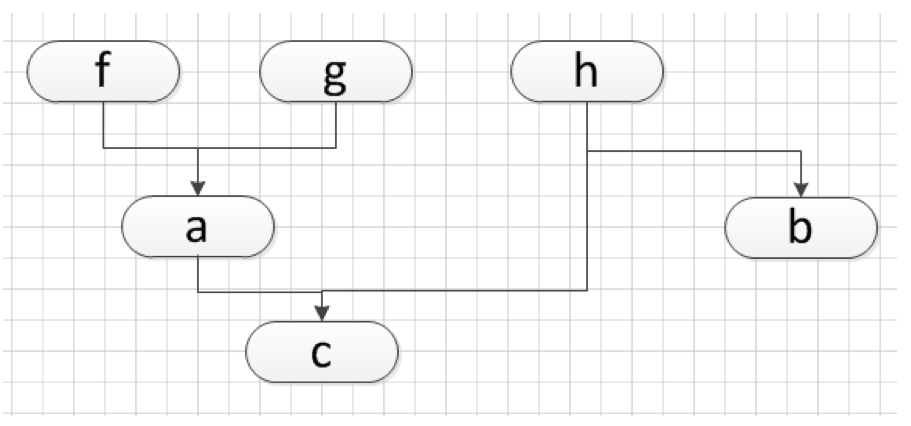
\includegraphics[scale=0.3]{flow.png}
\end{center}

We should only include formulae that belongs to functions that are
actually used. For example, to prove $a$'s contract, we should only
include $f$ and $g$ translations, and we would ask equinox:
$$ \dtrans{f},\dtrans{g},\dtrans{a},\ctrans{f},\ctrans{g} \vdash
\ctrans{a}$$


\section{Correctness of the translation}
For the translation to be useful, $\trans{M} \vdash \ctrans{f \in c} $
should imply that $f \in c$.


\section{Higher-orderness}
\label{ho}
Our current translation only considers fully applied functions and
first-order functions. For example, so far, we cannot give any
contract to $map$ because it would involve quantifying over a
function, a thing that is not first-order.

There is a possible workaround, which involves the ``app'' function
defined in our first-order logic. Assume we have a function $f$ that
is not fully applied somewhere in a module. We create the term
$f\_ptr$ which relates to $f$ by the equations given in figure~\ref{ho-fig}

This way, we can emulate quantification over function by quantifying
on their $ptr$ counterpart.


\begin{figure*}
$$ \forall x_1,\dots,x_n.~\full{f}(x_1,\dots,x_n) = f~x_1~x_2~\dots~x_n$$
$$ \cf{f} \tot \forall x_1,\dots,x_n.~\cf{x_1} \land \dots \land \cf{x_n} \to \cf{\full{f}(x_1,\dots,x_n)}$$
$$\forall g,x.~\cf{f} \land \cf{x} \to \cf{g~x}$$
\caption{Encoding of higher-orderness}
\label{ho-fig}
\end{figure*}

\section{Experiments}
That's how we roll.

\begin{figure*}
\begin{center}
    \begin{tabular}{l|c|c|c|c|c}
      Problem & Equinox & Equinox (+ weak) & SPASS & Vampire & E \\
      \hline
      Add.hs & 0.25 & 0.08 & 0.04 & 0.12 & 0.05\\
      BinaryTree.hs & 0.45 & 0.2 & 0.04 & 0.01 & 0.04 \\
      Branch.hs & 0.27 & 0.40 & 0.04 & 0.01 & 0.03 \\
      Copy.hs & 0.86 & 0.09 & 0.03 & 0.01 & 184.3 \\
      Head.hs & 0.32 & 0.29 & 0.03 & 0.03 & 4.2 \\
      Implies.hs & 3.24 & 0.32 & 0.06 & 0.02 & 0.11 \\
      Map.hs & 2.47 & 0.14 & 0.92 & 1.02 & $>$300 \\
      Mult.hs & $>$300 & 0.41 & 0.05 & 0.22 & 11.71 \\
      Multgt.hs & $>$300 & 1.24 & 0.62 & 1.31 & $>$300 \\
      NatEq.hs & 203.12 & 0.33 & 0.02 & 0.03 & 0.343 \\
      Odd.hs & 0.42 & 1.17 & 0.06 & 0.03 & $>$300 \\
      Reverse.hs & 72.32 & 0.12 & 0.05 & 0.02 & 0.038 \\
      Simple.hs & 0.07 & 0.04 & 0.01 & 0.01 & 0.022 \\
      Test.hs & 7.76 & 2.86 & 0.08 & 0.05 & $>$300 \\
      Test2.hs & 5.63 & 0.09 & 0.07 & 0.01 & 1.02 \\
    \end{tabular}
\end{center}
\caption{Comparison (in seconds) with other theorem provers}
\label{comparison}
\end{figure*}

\end{document}
